Neste apêndice, mostram-se os principais resultados da análise descritiva de dados. 
% TODO: colocar descrição do que é encontrado aqui

\section{Atributos Eliminados devido a Missing Values} \label{graf_miss_value}
\par Eliminaram-se os atributos raça e tipo da escola, pela quantidade de missing
values ser superior a 40\%.  A Figura \ref{atr_race} mostra o gráfico de barra para o
atributo raça, enquanto que a Figura \ref{atr_school_type} mostra o gráfico de barra
para o atributo tipo da escola.  
    % raça
    \begin{figure}[!ht]
        \caption{Gráfico de Barra para Atributo Raça}
        \centering
        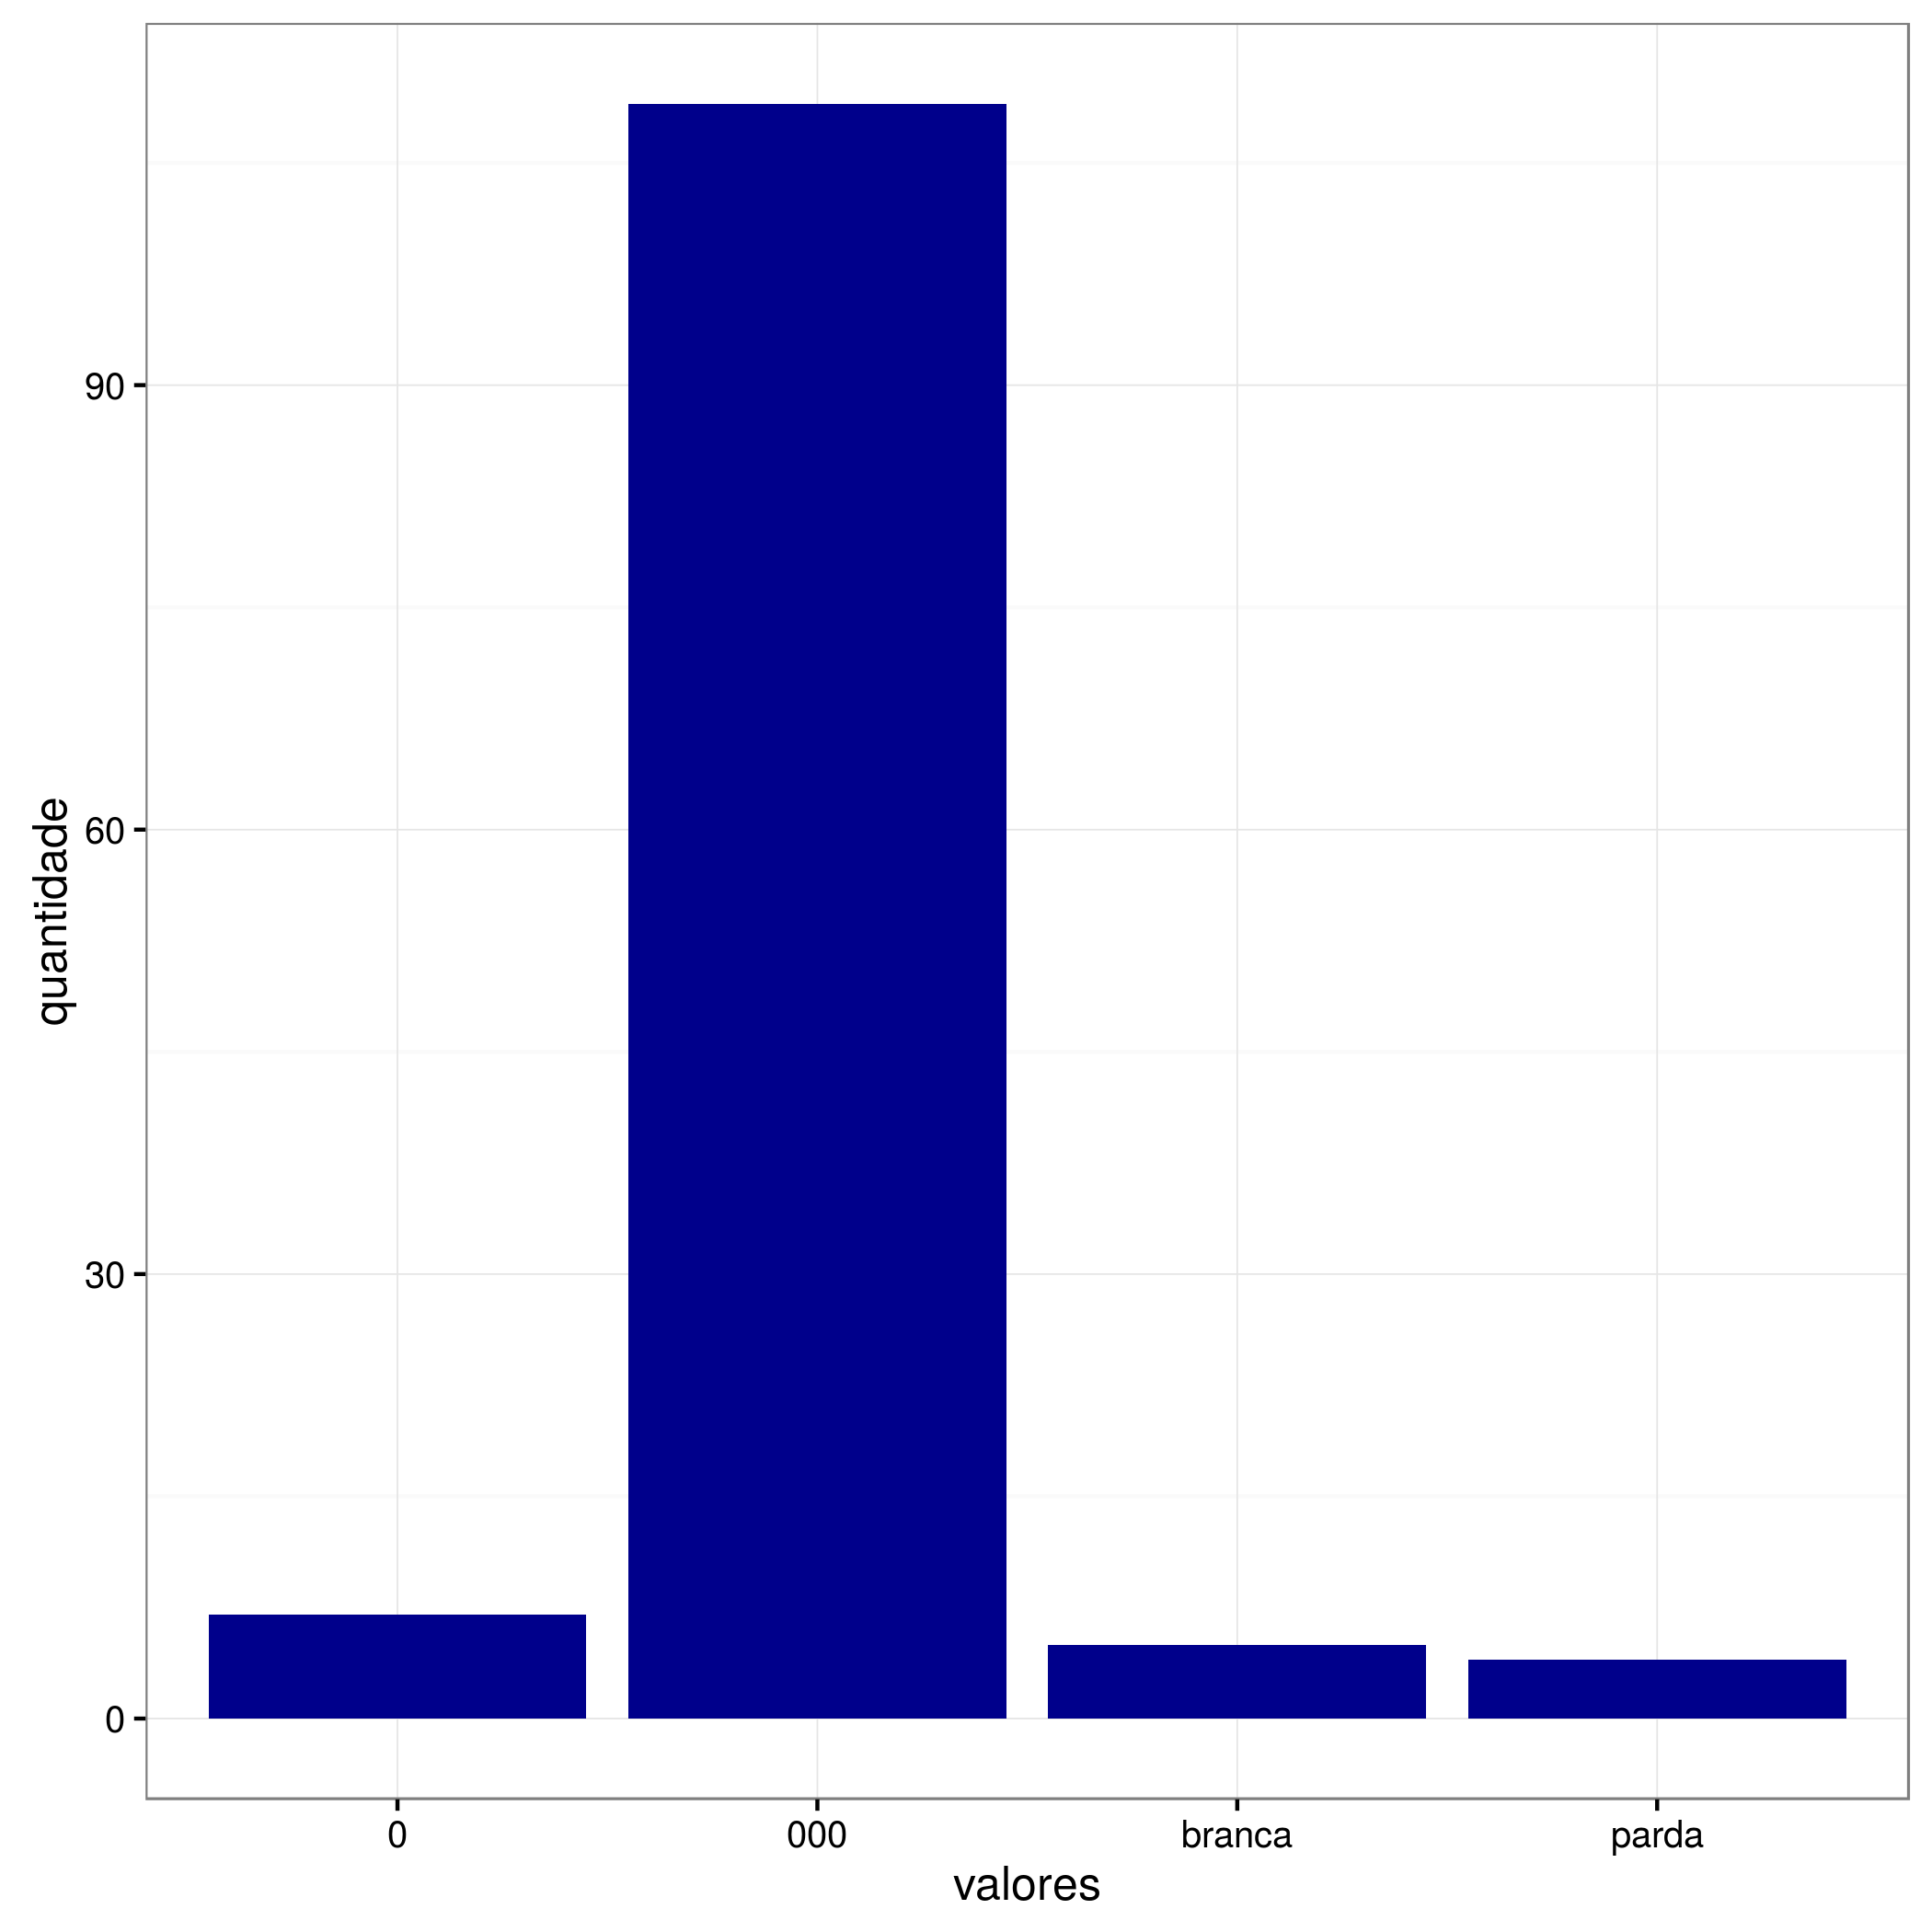
\includegraphics[width = 10cm]{all_students/race.png}
        \label{atr_race}
    \end{figure}

    % tipo da escola
    \begin{figure}[!ht]
        \caption{Gráfico de Barra para Atributo Tipo da Escola}
        \centering
        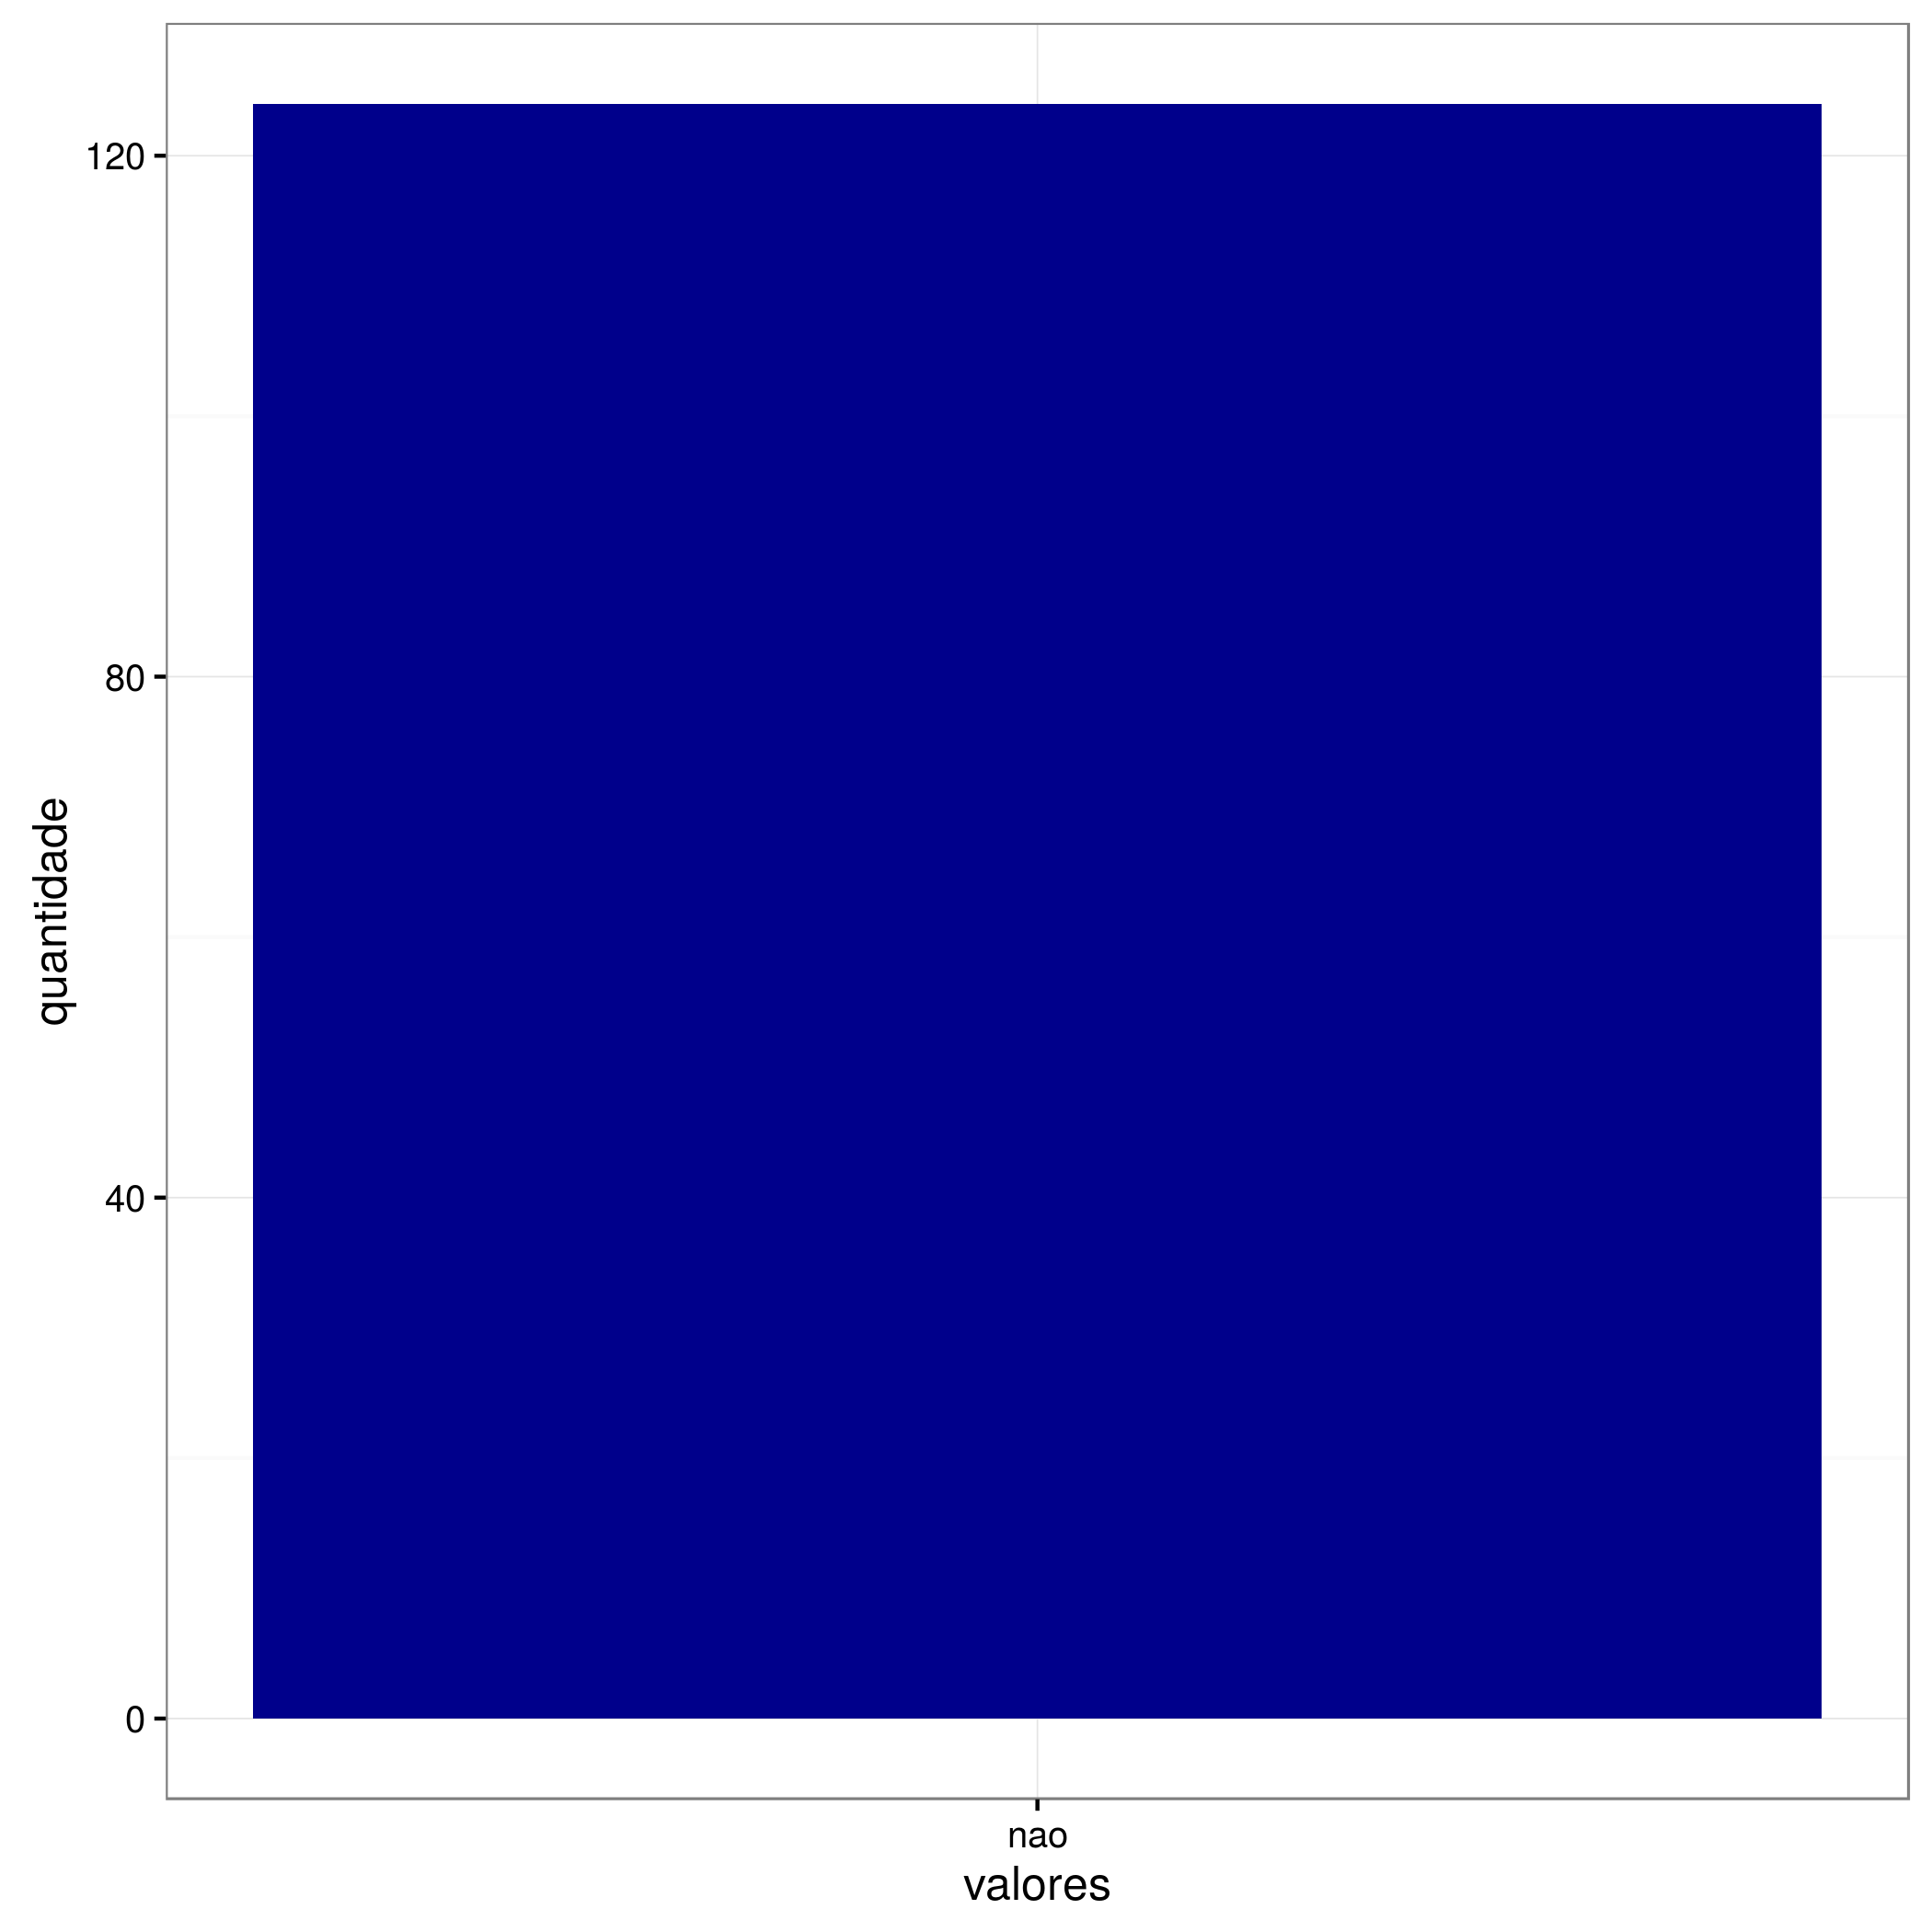
\includegraphics[width = 10cm]{all_students/school_type.png}
        \label{atr_school}
    \end{figure}

Conforme já dito, em ambos os casos, observam-se uma grande quantidade de valores
faltantes, de modo que tais atributos foram retirados de análises posteriores. 

\section{Impacto do Curso e Idade na Separação de Variáveis: Surgimento das 4 Bases
de Dados} \label{justificativa_4_base_dados}
Na análise preliminar por meio de estatística descritiva, analisou-se como a
distribuição dos atributos era afetada pelo curso do aluno, tendo-se constatado que a
influência do fator curso era bastante significativa. 
%Percebe-se isso, por exemplo, na tabela \ref 

% todo
%\begin{table}
%\begin{center}
%\begin{tabular}[c]{| c | c |}
%    \hline
%    Curso & Percentagem capaz de Formar \\
%    \hline
%\end{tabular}
%\end{center}
%\caption{Percentagem de Alunos Capazes de Formar, de Acordo com o Respectivo
%    Curso}
%\end{table}

\par Além do curso, a análise descritiva mostrou que a taxa de alunos que conseguem
formar é consideravelmente menor para alunos mais velhos. 
%A tabela \ref{} indica isso 

% todo: colocar tabela 

\section{Mudança de Valores de Atributos}
Conforme mencionado, os atributos forma de entrada e forma de saída tiveram seus
valores menos comuns agrupados em certas categorias. O gráfico de barra para o
atributo forma de ingresso, com seus valores originais, é mostrado na Figura
\ref{atr_way_in_org}. 
Por questões de legibilidade, a legenda no gráfico foi encurtada. Seu significado é
apresentado a seguir: 

    \begin{itemize}
    \item \texttt{vest}: Ingresso via Vestibular
    \item \texttt{ci}: Ingresso via Convênio-Int
    \item \texttt{to}: Ingresso via Transferência Obrigatória
    \item \texttt{to}: Ingresso via Transferência Obrigatória
    \item \texttt{ac}: Ingresso via Acordo Cultural PEC
    \item \texttt{ca}: Ingresso via Convênio Andifes
    \item \texttt{mc}: Ingresso via Matrícula Cortesia
    \item \texttt{tf}: Ingresso via Transferência Facultativa
    \item \texttt{ppp}: Ingresso via PEC-G Peppfol
    \item \texttt{pdcs}: Ingresso pois é portador de diploma de curso superior
    \item \texttt{vmc}: Ingresso via Vestibular para Mesmo Curso
    \end{itemize}

    \begin{figure}[!ht]
    \caption{Gráfico de Barra de Todos os Alunos, para o Atributo Forma de Ingresso}
    \centering
    \includegraphics[width = 10cm]{all_students/way_in.png}
    \label{atr_way_in_org}
    \end{figure}

O gráfico de barra para o atributo forma de saída, com seus valores originais, é
mostrado na Figura \ref{atr_way_out_org}. 
Por questões de legibilidade, a legenda no gráfico foi encurtada. Seu significado é
apresentado a seguir: 

    \begin{itemize}
    \item \texttt{dec}: Ex-Aluno pelo Decreto 477
    \item \texttt{deslg}: Saída por desligamento
    \item \texttt{form}: Saída pois conseguiu formar
    \item \texttt{mrr}: Saída por falecimento
    \item \texttt{null}: Saída por anulação de registro
    \item \texttt{trnsf}: Saída devido à Transferência
    \item \texttt{vest}: Saída devido à novo vestibular
    \end{itemize}

    \begin{figure}[!ht]
    \caption{Gráfico de Barra para Atributo Forma de Saída}
    \centering
    \includegraphics[width = 10cm]{all_students/way_out.png}
    \label{atr_way_out_org}
    \end{figure}

\section{Gráficos de Barra e Histogramas} \label{graf_bar_hist}

